\section{General Overview of the Simulation Output}
\label{sec:general-overview-of-simulation-output}
First, let us describe the outcome of the simulation framework which is visualized in the figure \ref{fig:single-simulation-example}.
The simulation framework provides this graph for each possible simulation.

The graph's headline explains what setup parameters for the trust model were used. In the case of \ref{fig:single-simulation-example} Fides used $MaxConfidenceTIEvaluation$ (\ref{subsec:MaxConfidenceTIEvaluation}) for evaluating interactions between the peers.
For aggregating threat intelligence, Fides used the aggregation described in the section \ref{sec:network-intelligence-aggregation}.
Local Slips instance behaved like confident correct peer outlined in the section  \ref{subsubsec:confident-correct-peer}.

\begin{figure}
    \centering
    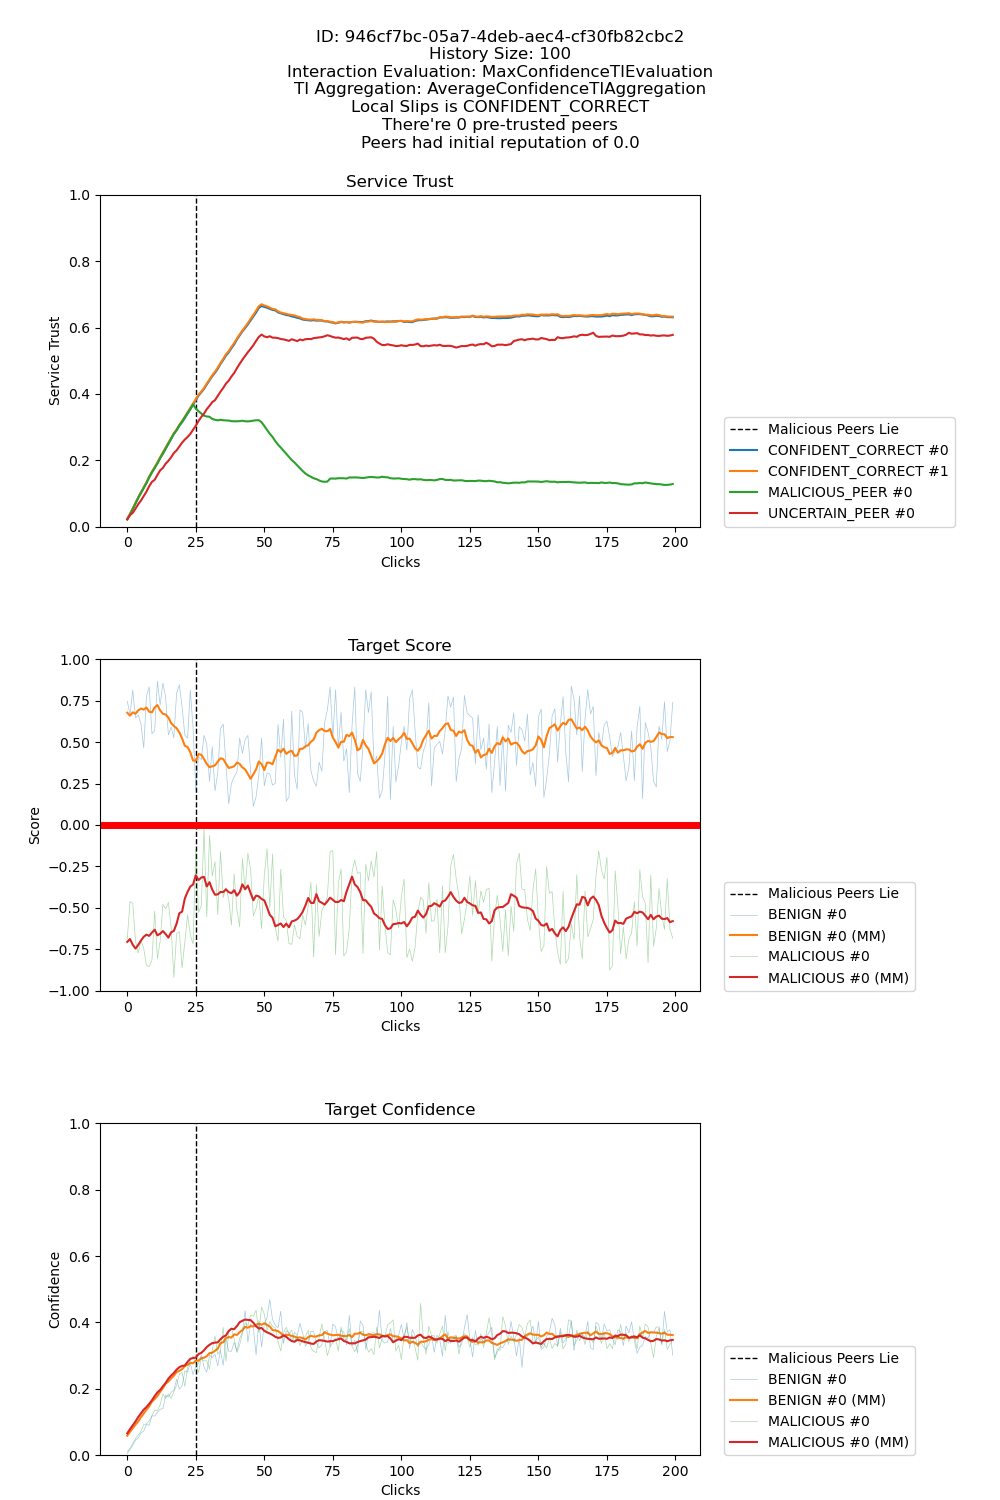
\includegraphics[width=1.0\textwidth]{assets/example_evaluation.png}
    \caption{Example of a single simulation}
    \label{fig:single-simulation-example}
\end{figure}

The first graph in the figure \ref{fig:single-simulation-example} is the development of \textit{service trust} $st_{i, j}$ (\ref{subsec:service-trust}) on the vertical axis during the \textit{time} on the horizontal axis. As mentioned in the section \ref{sec:environment-simulation}, the time is measured in \textit{clicks}.
One can see multiple peers that were involved in the simulation and their respective behavior. All possible behaviors are described in the section \ref{sec:peers-behavioral-patterns}.
There were four different peers that were communicating with the local instance of Fides, two of them were \textit{confident correct}, one was an \textit{uncertain peer} and the last one was a \textit{malicious peer}.

The dotted line separates the period on all graphs, where the malicious peers are gaining the initial service trust and the period when the malicious peers lie.
In the case of figure \ref{fig:single-simulation-example} this happened at click 25 when the malicious peers started lying.

The second graph in the figure \ref{fig:single-simulation-example} shows the \textit{target score} during the time (\textit{clicks}).
Target score $S^{k}_{T}$ (\ref{sec:network-intelligence-aggregation}) is the part of the aggregated network threat intelligence, that was computed from the scores and confidences provided by each peer.
The score was calculated by Fides at click $k$ for target $T$.

The score graph contains two different targets, one that is according to the ground truth malicious and the second, that was benign.
We also included moving average value within the window of 10 clicks to make the graph clear.

The last, third graph, displays the aggregated confidence $C^{k}_{T}$ (\ref{sec:network-intelligence-aggregation}) during the time (\textit{clicks}).
The graph is similar to the score, we include raw values for each time window and target as well as the moving average within the window of 10 clicks.

One can see that the Fides was clearly able to identify that malicious peer started to lie after click 25 because of the service trust $st^{k}_{i,j}$ for this peer that fell down almost instantly.
At the same time, we can see that on the score graph, the $S^{k}_{T}$ for both targets were skewed and started to get closer to $0$ because the malicious peer had already gained service trust and thus the threat intelligence provided by it had an impact on the final $S^{k}_{T}$.
However, after Fides figured out, that the peer is lying, it lowered its service trust for this peer and the score started to recover closer to the baseline.